\documentclass[review,authoryear]{elsarticle}
\usepackage{amssymb}
\usepackage{graphicx}
\usepackage{subfigure}
\usepackage{latexsym}
\usepackage{amsfonts}
\usepackage{amsmath}
\usepackage{lineno}
\usepackage[para]{threeparttable}
\usepackage{rotating}
%\usepackage{graphicx}
\usepackage[graphicx]{realboxes}
\graphicspath{ {./figures/} }
\newcommand{\esysparticle}{\textit{Esys-Particle }}
\journal{International Journal of Coal Geology}
\usepackage{booktabs}
\begin{document}
\begin{frontmatter}

\title{Numerical Investigations on the Impact of Cleat Characteristics on Elastic Anisotropy in Coal Seam Gas Reservoirs}
\author[UQ]{Jinfang Gao\corref{CA}}
\ead{j.gao1@uq.edu.au}

\author[UQ]{Lutz Gross}
\ead{l.gross@uq.edu.au}

\author[UQ]{Steve Tyson}
\ead{s.tyson@uq.edu.au}

\author[UQ]{Tom Rufford?}
\ead{}


\address[UQ]{Centre for Geoscience Computing, School of Earth Sciences,
The University of Queensland, St. Lucia, Brisbane, QLD \emph{4072}, Australia}

\cortext[CA]{Corresponding author.}

\begin{abstract}
Coal seams are embedded into other sedimentary structures, such as sands, clays and shales. In coal seam gas reservoir engineering, structures such as layering, fractures, cleat orientations, porosity and fluids within the cleats have an important effect on production. The interpretation of 3D seismic surveys in terms of these fractures characteristics is of great interest.

Weak anisotropy is commonly described using Thomsen-style parameters. From seismic survey data, values for Thomsen-style parameters are determined, 
usually through non-hyperbolic normal moveout (NMO) and azimuth gathers. The interpretation of the parameters in terms of fracture characteristics 
is based on restrictive assumptions; sparse, non-interacting, disk-shaped fractures are commonly assumed in cases where fracture geometry is not required. 
This paper investigates the effect of 3D fracture geometry in coal seams on the effective 3D anisotropic elasticity parameters using a numerical approach. 
We show some first results to verify existing, commonly used elastic models for fractured media, derived under restrictive assumption and then test their validity for more 
realistic scenarios; fracture distributions and densities, and material-filled cleats. Our study will help to provide a more reliable interpretation of Thomsen-style parameters obtained from seismic survey data. 

The impact of cleats, and other small-scale structures, on the elastic properties of coal is investigated using the discrete element method (DEM). The method is capable of simulating complex fracture distributions, surface roughness and orientations on different spatial scales. Firstly, DEM is calibrated by performing uni-axial compression testing and shearing testing on a virtual coal sample, to determine values for macroscopic model parameters for intact coal. Then, cleats with different fracture densities and occupying materials are added. From these tests, we are able to validate commonly-used elasticity models for fractured media (e.g., Linear-slip models), which is of first order in fracture density. 

\end{abstract}


\begin{keyword}
Coal seam gas reservoirs; Fractures and cleats; 3D anisotropy; Elasticity tensor; Stiffness; Discrete Element Method (DEM)
\end{keyword}

\end{frontmatter}

\linenumbers

%% main text
\section{Introduction: Origin of coal samples, geology background, fracture styles}
Coal seam gas (CSG) reservoirs comprise fractured coal and non-coal, less-fractured inter-burdens. Such sedimentary structures together with the fracture-filled fluids have significantly affected the gas production in coal seams such as leaking, fines induced blockage and contamination, see \cite{thomas1983fractured}, \cite{clarkson2006production}, \cite{golding2013stable} and \cite{flottman2013influence}. Interpretation and measurement of geometric formation characteristics (e.g. 3D anisotropy) in terms of elasticity tensor or stiffness matrix is thus of great importance for operation of CSG reservoirs.

The analysis of seismic surveys can provide 3D formations characteristics, e.g. see \cite{grechka19983}; \cite{schoenberg1995seismic}; \cite{biondi20063d}; \cite{grechka2006effective}. Thomsen-style parameters are used to describe seismic 3D azimuthal anisotropy. They can be determined through non-hyperbolic normal moveout (NMO) analysis on azimuth gathers, e.g. see \cite{vermeer20023}; \cite{tsvankin2011seismology}. Together with a lithology analysis of well-logs, 
the 3D anisotropy is interpreted and upscaled to larger spacial scales vertically as well as horizontally. 
However the minimum  wavelengths used in seismic surveys are typically well above $1 m$, while the estimates of in-situ fracture apertures range from $0.001$ to $20 mm$ \citep{gamson1993coal}. As a consequence seismic survey analysis can provide effective elastic properties only in cases of fractured media such as coal that
show anisotropic properties following the fracture orientations. The effective elastic parameters are determined by the host rock as well 
as the fracture details (e.g. intensity, orientations, shapes and sizes, and fracture-filling materials).

Then, Aguilera et al. \citep{aguilera1998geologic} have found that natural fractures in subsurface systems usually occur in large populations or sets with similar orientations. According to this, linear-slip models and Hudson's model have been proposed and widely used for studying the effective parameters of fractured media.
The linear-slip models (see \cite{schoenberg1980elastic}, \cite{schoenberg1983reflection}) suggest treating fractures as aligned parallel planes regardless of their shapes and microstructures; while Hudson's model (see \cite{hudson1980overall}, \cite{hudson1981wave}) assumes the fractures as a set of sparse, non-interacting, parallel penny-shaped cracks. These cracks have similar shapes and sizes. Schoenberg and Douma's studies \citep{schoenberg1988elastic} have shown that these models share profound similarity in describing the formation matrix, dry fractures and fracture-filled fluids to model anisotropic, long-wavelength wave propagation. 

For a better interpretation, this paper numerically investigates the impact of fractures characteristics on 3D anisotropy and the host rock properties (e.g., anisotropic elasticity tensor or stiffness). In numerical modelling, the Discrete Element Method (DEM) is well established for simulating complex fracture distributions, surface roughness and orientations on different spatial scales. \esysparticle (see {launchpad.net/esysparticle}) is an open source implementation of the DEM for execution on desktop computers or multi-core supercomputers with Linux-based operating systems \citep{weatherley2013esys}. It supports parallelization using the Message Passing Interface (MPI) \citep{gropp1999using} to run simulations with several milions of particles on multi-core and multi-node computing infrastructures.
\esysparticle has successfully been applied to broad variety of areas including the simulation of brittle rock fractures and earthquake process (\cite{wang2008discrete}; \cite{weatherley2010scaling}; \cite{abe2012discrete}; \cite{mora2015lattice}). 

It is the objective of our study to develop a better understanding on how seismic anisotropy can be interpreted in terms of fracture intensity, geometry and filling. The starting point of our investigation is the Linear-slip models for crack induced, anisotropic weakening which has been developed for very restrictive assumption on the crack characteristics. The paper presents some first results on validating Linear-slip models using DEM based \esysparticle simulations and then investigates the impact of hight-density, interacting fractures as well as fracture filling on Thomsen-style parameters. 
The results show good agreement between DEM simulations and the Linear-slip models for sparse fractures 
but significant divergence between the two approaches can be observed for higher fracture intensities as 
expected.

\begin{figure}
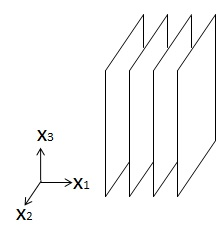
\includegraphics[scale=0.8]{./figures/HTI.jpg}
\centering
\caption{HTI medium with parallel vertical fracture planes normal to $x_1$ axis.}\label{FIG:HTI}
\end{figure}

\section{Anisotropy and Fracture-sets models:regarding distribution of parallel fractures}

In our investigations we focus on cases of (predominately) parallel fracture systems with a single fracture plane, see Figure~\ref{FIG:HTI}. At large scales, such a medium is described as a HTI medium. For the sake of a simpler presentation we assume that symmetry axes of the HTI media are aligned 
with the $x_{1}$ axes. The linear relationship between the symmetric stress tensor $\sigma_{ij}$ and the strain tensor $\varepsilon_{ij}$ 
for HTI media is written in the form:
\begin{equation}\label{EQ:STRESS-STRAIN}
\begin{array}{ccc}
\sigma_{11} = C_{11} \; \varepsilon_{11} +  C_{12} \; \varepsilon_{22} +  C_{12}\varepsilon_{33} \\
\sigma_{22} = C_{12} \; \varepsilon_{11} +  C_{33} \; \varepsilon_{22} +  C_{23}\varepsilon_{33} \\              
\sigma_{33} = C_{12} \; \varepsilon_{11} +  C_{23} \; \varepsilon_{22} +  C_{33}\varepsilon_{33} \\ 
\sigma_{23} = 2 C_{44}\varepsilon_{23} \\ 
\sigma_{13} = 2 C_{66}\varepsilon_{13} \\ 
\sigma_{12} = 2 C_{66}\varepsilon_{12} \\
\end{array}
\end{equation}
where $C_{ij}$ is elasticity tensor in Voigt notation:
\begin{equation}\label{EQ:ELASTENSOR}
  C_{ij} = \left[
  \begin{array}{cccccc}
 C_{11} & C_{12} & C_{12} & 0 & 0 & 0 \\
 C_{12} & C_{33} & C_{23} & 0 & 0 & 0 \\
 C_{12} & C_{23} & C_{33} & 0 & 0 & 0 \\
 0 & 0 & 0 & C_{44} & 0 & 0 \\
 0 & 0 & 0 & 0 & C_{66} & 0 \\
 0 & 0 & 0 & 0 & 0 & C_{66} 
\end{array}
  \right]
\end{equation} 
In the application case of a single reflector below the HTI medium, the entries of elastic tensor can  be determined from a normal moveout (NMO) velocity analysis, see \cite{Tsvankin1997b} and \cite{Tsvankin1997a}. For this analysis it is convenient to use so-called Thomsen-style parameters \citep{Tsvankin1997b}
 which are represent via the elasticity coefficients within the $x_{1}$-$x_{3}$ plane:
\begin{equation}\label{EQ:Thomsen:2}
\varepsilon^{(2)}=\frac{C_{11}-C_{33}}{2C_{33}} \mbox{, }
\gamma^{(2)}=\frac{C_{66}-C_{44}}{2C_{44}} \mbox{ and }
\delta^{(2)}=\frac{(C_{13}+C_{44})^2-(C_{33}-C_{44})^2}{2C_{33}\cdot(C_{33}-C_{44})}
\end{equation}
%\begin{equation}
%\eta^{(2)}=\frac{\varepsilon^{(2)}-\delta^{(2)}}{1+2\delta^{(2)}}
%\end{equation}

With the knowledge of density, the vertical P-wave ($V_{P}$) and S-wave ($V_{S}$) velocities, the entries in the HTI elasticity tensor $C_{ij}$ in Equation~(\ref{EQ:ELASTENSOR}) can be recovered from the Thomsen-style parameters.

To model fracturing within an isotropic medium the linear slip model is being used, see \cite{schoenberg1980elastic}. Under the assumption of parallel fractures
along the verticle direction $x_{2}$-$x_{3}$ plane, the weakness of the media stiffness is descibed using the weakness $\Delta_N$ (normal to the fracture plane) and $\Delta_T$ (tangential to the fracture plane) \citep{bakulin2000estimation}. With these quantities the elasticity tensor $C_{ij}$ of the fractured media is written as:
\begin{equation}\label{EQ:FRACTENSOR}
  C_{ij} = \left[
  \begin{array}{cccccc}
M(1-\Delta_N) & \lambda(1-\Delta_N) & \lambda(1-\Delta_N) & 0 & 0 & 0 \\
\lambda(1-\Delta_N) & M(1-r^2\Delta_N) & \lambda(1-r\Delta_N) & 0 & 0 & 0 \\
\lambda(1-\Delta_N) & \lambda(1-r\Delta_N) & M(1-r^2\Delta_N) & 0 & 0 & 0 \\
 0 & 0 & 0 & \mu & 0 & 0 \\
 0 & 0 & 0 & 0 & \mu(1-\Delta_T) & 0 \\
 0 & 0 & 0 & 0 & 0 &  \mu(1-\Delta_T)
\end{array}
  \right]
\end{equation}  

where $\lambda$ and $\mu$ are the first Lame parameter and the shear modulus, respectively. $M = \lambda + 2\mu$, $r = \frac{\lambda}{M}$ and $g = \frac{\mu}{M}$. The fracture model by ~\cite{bakulin2000estimation} for parallel, independent cracks is:
\begin{equation} \label{EQ:DELTAN}
  \Delta_N = \frac{4\,e}{3\, g(1-g)}
  \end{equation}
and 
\begin{equation} \label{EQ:DELTAT}
\Delta_T = \frac{16\, e}{3(3-2g)
}
\end{equation}
where $M'$ and $\mu'$ are the P-wave modulus and shear modulus of the fracture-filled material. The semiminor axes and  semimajor axes of the spheroid-shaped cracks are denoted by $c$ and $a$, respectively. The quantity $e$ gives the fracture density which is the product of the average number of cracks per volume and the fractured volume ($a^3$).
$\varepsilon^{(2)}$ and $\delta^{(2)}$ are hereby correlated with small $\Delta_N$ and $\Delta_T$ as:
\begin{equation}\label{EQ:THOMSEN-4}
  \varepsilon^{(2)} = -2g(1-g)\Delta_N \mbox{ and }   \delta^{(2)} = -2g[(1-2g)\Delta_N+\Delta_T]
\end{equation}
%\begin{equation}\label{EQ:THOMESON-5}
% \gamma^{(2)} = -\frac{\Delta_T}{2}
% \end{equation}
Values for $\delta^{(2)}$ and $\varepsilon^{(2)}$ are obtained by non-hyperbolic NMO analysis which allows to recover values for the 
weakening coefficients $\Delta_N$ and $\Delta_T$ if the value $g$ for the unfractured material is known (e.g. from well logs).   
It is the objective of the investigation in the paper to develop some understanding how Thomsen-style parameters are controlled by fracture density, shape and fillings beyond the assumptions of the Linear-slip models ~(\ref{EQ:DELTAN}) and~(\ref{EQ:DELTAT}) in particular 
for the case of high fracture density with interacting fractures.   

\begin{figure}[t]
\centering
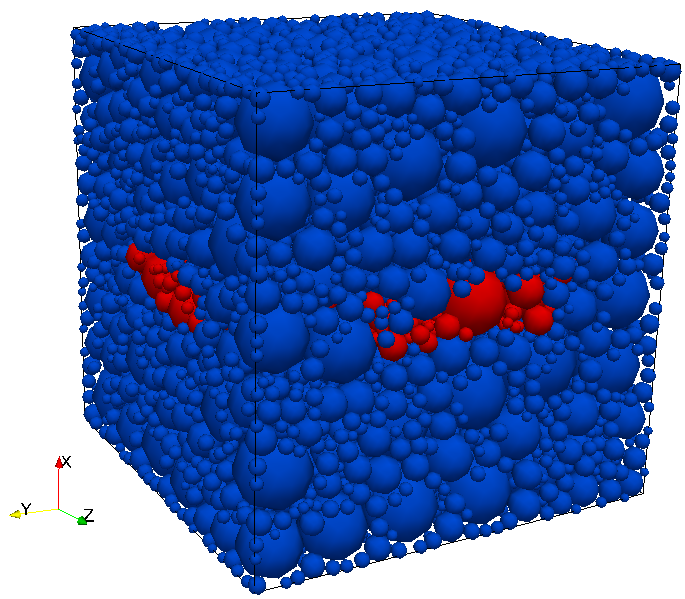
\includegraphics[scale=0.2]{./figures/particle.jpg}
\caption{A representative sample of medium with a single horizontal fracture using DEM. 
Particles in the background media and the fracture filling are coloured in blue and red, respectively.\label{FIG:particle}}
\end{figure}


\section{Discrete Element Method and \esysparticle}
The Discrete Element Method (DEM) \citep{cundall1979discrete} is a numerical method for simulating the dynamics of brittle-elastic and 
granular materials with discontinuity due to fractures. Over the past decades it has been widely used for addressing engineering problems especially in granular flows, powder mechanics and rock mechanics, for instance see \cite{pande1990numerical}, \cite{langston1995discrete}, \cite{martin2003study} and \cite{jing2007fundamentals}. 
In the basic idea of DEM, materials are represented as assemblies of typically spherical particles of different sizes. 
In the simulations used in this paper, the domain is a box covering a representative sample of the fractured media, see Figure~\ref{FIG:particle}. 
In this picture, particles coloured in blue represent particles in the background medium (a $5 cm$ cubic) while particles coloured in red represent particles filling fractures. The particle size in Figure~\ref{FIG:particle} ranges from a maximum size of $1.0 mm$ to a minimum size of $0.1mm$ resulting in a porosity of the medium is $0.23$. 
The miminum particle size controls the porosity of the background medium, where a smaller miminum size relates to a relatively lower porosity. 

At each time step, particles are moving according to the Newton's second law of motion while each particle interacts with its neighbouring particles or other objects, such as planar walls. At contacts simplified force-displacement interaction laws are applied to define contact forces from displacements \citep{cundall1979discrete}. DEM describes four types of particle interactions including normal forces, shearing forces, bending moment and twisting moment. The increment in 
normal force $\Delta F_{(n)ij}$ and shear force $\Delta F_{(s)ij}$ acting between particles $i$ and $j$ is then defined according to the force-displacement law:
\begin{equation}\label{EQ:DEM:1}
  \Delta F_{(n)ij} = k_{(n)ij}\Delta \delta_{ij} \mbox{ and } \Delta F_{(s)ij} = k_{(s)ij}\Delta_{ij} 
  \end{equation}
where the distance overlap $\Delta \delta_{ij}$ is found when the two particles $i$ and $j$  are pushed towards each other along the normal direction, and the $\Delta_{ij}$ is the distance displacements of these particles in the tangent direction. $k_{(n)ij}$ and $k_{(s)ij}$ are the normal and shearing stiffness of the assembly of these particles, which are calculated using Young's modulus $E$ and Poisson's ratio $\nu$. In this paper, these parameters are simply defined as:
\begin{equation}\label{EQ:DEM:2}
  \Delta k_{(n)ij} = \frac{E_{dem}}{3(1-2\nu_{dem})} \mbox{ and } \Delta k_{(s)ij} = \frac{\Delta k_{(n)ij}}{2(1+\nu_{dem})} 
  \end{equation}
It is pointed out that the Young's modulus and Poisson's ratio in Equation~(\ref{EQ:DEM:2}) are local microscopic quantities for the DEM modelling, which differ from the macroscopic elastic properties of a sample as defined in Equation~(\ref{EQ:FRACTENSOR}). Appropriate values for the microscopic properties need to be determined from the calibration,  see Section~\ref{SEC:CALI}.

A different set of local microscopic Young's modulus $E'_{dem}$ and Poisson's ratio $\nu'_{dem}$ is used for describing fracture filling materials (e.g. fluids) from the background medium. $k'_{(n)ij}$ and $k'_{(s)ij}$ are the normal and shearing stiffness for the filling materials, which is defined in Equation~(\ref{EQ:DEM:1}). In DEM, the assumption is applied that the time step is sufficiently small such that disturbances only propagate from one particle to its immediate neighbours 
within one time step. Besides, the velocities and accelerations are assumed to be constant through this evolution step. 
Stress or strain is imposed at the boundary, and the equilibrium force and displacement are calculated from the disturbances originating at the boundary. 
The translations $\ddot{\vec{r}}_{i}$ acceleration of motion of particle $i$ is calculated using the Newton's second law of motion:
\begin{equation}\label{EQ:TRANS}
  m_{i}\ddot{\vec{r}}_{i}=\sum\limits_{j}{\Delta F_{ij}}
\end{equation}
where $m_{i}$ is the mass of particle $i$. $\sum\limits_{j}{\Delta F_{ij}}$ is the resultant force (Equation~(\ref{EQ:DEM:1})) acting on the particle $i$, and the sum is taken over all neighbouring particles. The particle velocities and positions are then updated according to an explicit finite difference integration scheme \citep{munjiza2004front}. 

For our investigations we use the \esysparticle DEM code (\cite{weatherley2013esys}; \cite{wang2008discrete}; \cite{griffa2011vibration}; \cite{abe2012discrete}; \cite{mora2015lattice}). The core of the \esysparticle is a modular, object-oriented DEM simulation engine. In \esysparticle, particles may have up to three translational 
as used in the investigations of this paper but also support three rotational degrees of freedom as well as thermal properties. 
An explicit first-order finite difference time integration scheme is employed and a Verlet list neighbour search algorithm is also implemented for detecting neighbouring particles and a variety of interaction laws are implemented for bonded or unbounded interactions between particles. The \esysparticle DEM code has been implemented on supercomputing platforms for big data processing and calculations, which is highly on demand in our study. 

\section{Simulations}\label{SEC:MEDIA}

\begin{figure}[t]
\subfigure[Isotropic virtual sample]{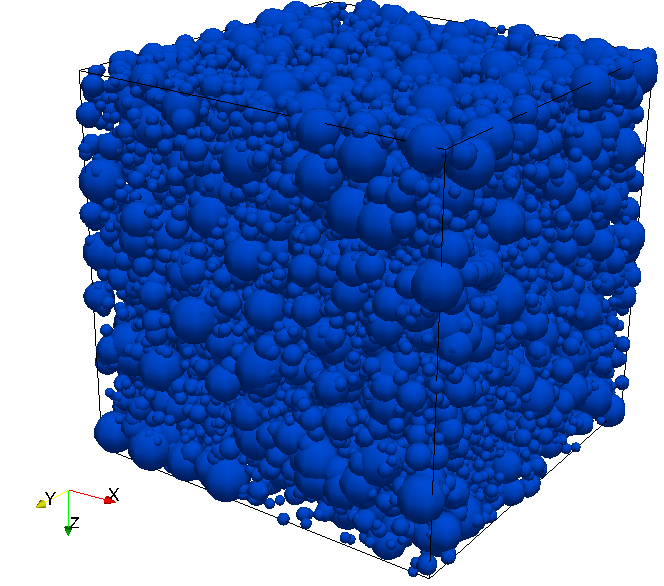
\includegraphics[scale=0.2]{./figures/frac0.jpg}}
\subfigure[Uni-axial compression]{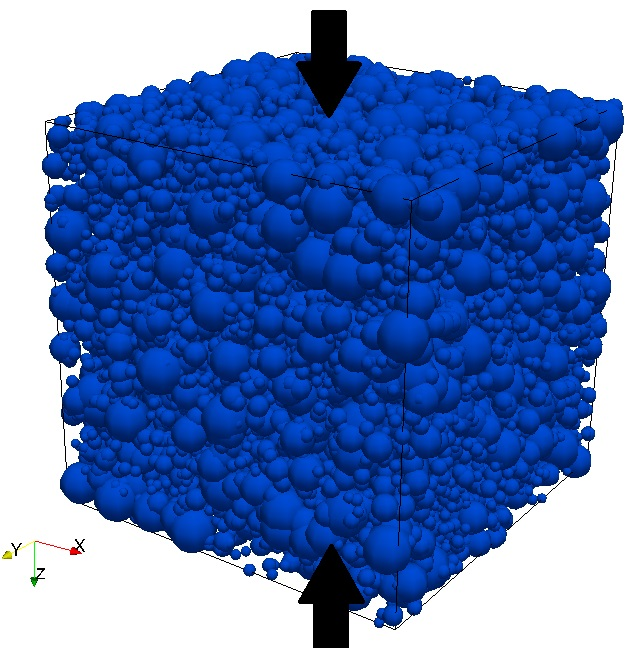
\includegraphics[scale=0.26]{./figures/compression.jpg}}
\subfigure[Shear test]{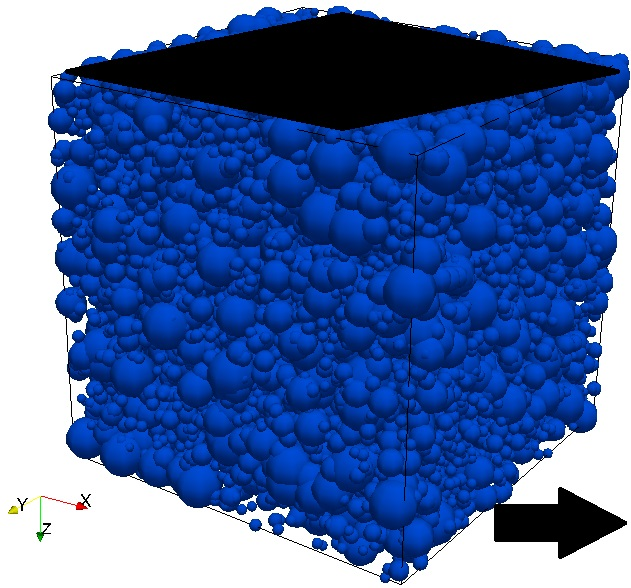
\includegraphics[scale=0.26]{./figures/shear.jpg}}
\centering
\caption{Calibration test configurations.}\label{FIG:GEOMETRY}
\end{figure}

\begin{figure}
\subfigure[Uni-axial compression ($\phi = 0.23$)]{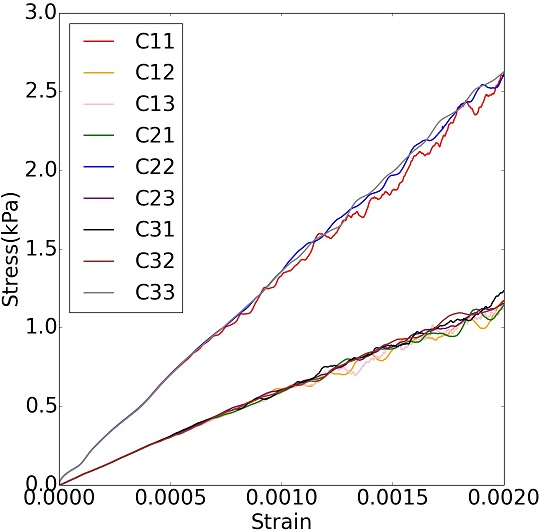
\includegraphics[scale=0.4]{./figures/frac0-same-low.jpg}\label{FIG:FRAC0a}}
\subfigure[Shear test ($\phi = 0.23$)]{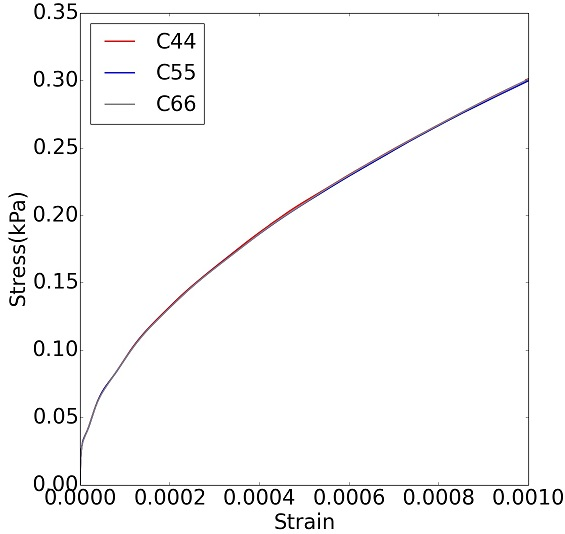
\includegraphics[scale=0.4]{./figures/frac0-same-low-shear.jpg}\label{FIG:FRAC0b}}
\subfigure[Uni-axial compression ($\phi = 0.30$)]{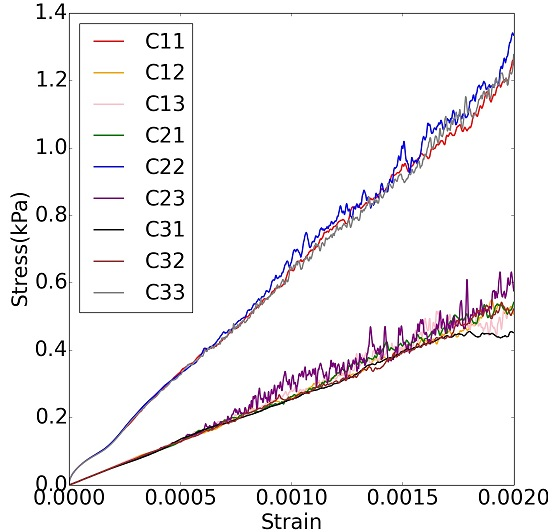
\includegraphics[scale=0.4]{./figures/frac0-same-hig.jpg}\label{FIG:FRAC0c}}
\subfigure[Shear test ($\phi = 0.30$)]{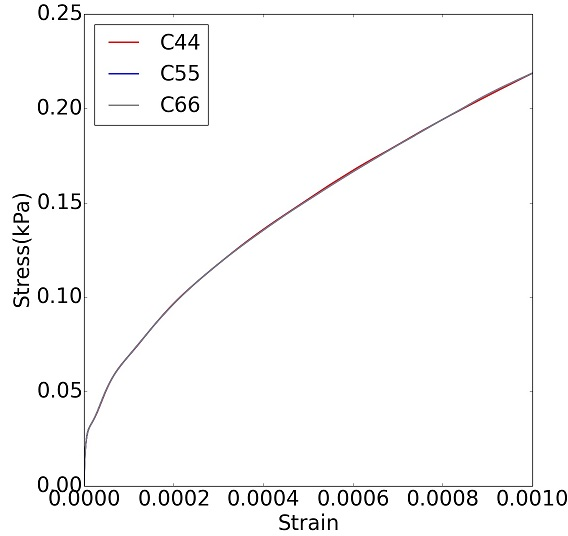
\includegraphics[scale=0.4]{./figures/frac0-same-hig-shear.jpg}\label{FIG:FRAC0d}}
\centering
\caption{Results for calibration testing on isotropic medium.}\label{FIG:FRAC0}
\end{figure}


\subsection{Calibration}\label{SEC:CALI}
Firstly, the \esysparticle model is calibrated through a uni-axial compression test and a shear test on an isotropic unfractured sample (edge length $5cm$, see Figure~\ref{FIG:GEOMETRY}). 
All tests are conducted in three directions to get all elasticity coefficient $C_{ij}$. 
For DEM modelling parameters, the local microscopic Young's modulus $E_{dem}$ is set as $3 MPa$ and the Poisson's ratio $\nu_{dem}$ is set as $0.25$. 
The largest particle size is $1.0 mm$ and the smallest particle size is $0.1 mm$, giving a porosity of $\phi = 0.23$. It is pointed out that 
for isotropic medium $\Delta_N = \Delta_T$ = 0 in equations~(\ref{EQ:DELTAN}) and~(\ref{EQ:DELTAT}).

\begin{table}
\centering
\caption{Model calibration results. $E_{mac}$ and $\nu_{mac}$ are referring to macroscopic Young's modulus and Poisson's ratio, respectively. }
\begin{threeparttable}[b]
\begin{tabular} {lrr}
%\begin{tabular}{p{2cm}p{4cm}p{4cm}}
\hline\hline 
 \multicolumn{3}{c}{Isotropic sample} \\
 \hline
Value\tnote{1} & $\phi=0.23$ & $\phi=0.30$ \\
\hline
$C_{11}$ 		& 1.309 & 0.613 \\
$C_{12}$ 		& 0.587 & 0.269 \\
$C_{23}$ 		& 0.587 & 0.269 \\
$C_{33}$ 		& 1.309 & 0.613 \\
$C_{44}$ 		& 0.361 & 0.172 \\
$C_{66}$ 		& 0.361 & 0.172 \\
$E_{mac}$  	    & 0.946 & 0.449 \\
$\nu_{mac}$  	& 0.310 & 0.305 \\
\hline    
\bottomrule
\end{tabular}\label{TABLE:ISOTROPIC}
\begin{tablenotes}
      \small
      \item [1] The unit for $C_{ij}$ and $E_{mac}$ is $MPa$.
	\end{tablenotes}
\end{threeparttable}
\end{table}

Figure~\ref{FIG:FRAC0} compare the stress and strain in the uni-axial compression tests (Figure~\ref{FIG:FRAC0a}) and shearing tests (Figure~\ref{FIG:FRAC0b}).
The elasticity coefficients are calculated by the slope of the stress and strain. In particular, all the slopes are calculated from the status (strain $\geq 0.0005$) for reducing the effect of initial particles settings. 
The isotropy is obviously observed as $C_{11}$= $C_{22}$ = $C_{33}$, $C_{12}$ = $C_{13}$ = $C_{23}$ and $C_{44}$ = $C_{55}$ = $C_{66}$. For details, the values of all elasticity coefficients are shown in Table~\ref{TABLE:ISOTROPIC}. Notice that $C_{33}$ = $C_{23}$ + $2C_{44}$ as expected for an isotropic medium. The macroscopic Young's modulus $E_{mac}$ and Poisson's ratio $\nu_{mac}$ are then calculated as $0.946 MPa$ and $0.310$, respectively. Notice that these macroscopic values are different from the corresponding microscopic values $E_{dem}$ ($=3 MPa$) and $\nu_{dem}$ ($=0.25$). The macroscopic value $E_{mac}$ for the Young's modulus does in fact scale with the microscopic Young's modulus $E_{dem}$. Therefore, a DEM model can easily be scaled to match a given macroscopic value $E_{mac}$ for the Young's modulus using the value from Table~\ref{TABLE:ISOTROPIC}.

Besides, we also compare the porosity effect of background medium on the testing (Figure~\ref{FIG:FRAC0c} and~\ref{FIG:FRAC0c}). The porosity of the background medium is $\phi = 0.30$ by increasing the smallest particle size to $0.2mm$. In this higher porosity case, elasticity 
coefficients tested are smaller than those for the case $\phi=0.23$, which is caused by the weakening due to larger pore space. 
The higher porosity also causes more stress fluctuation during the numerical testing (see comparison of Figure~\ref{FIG:FRAC0a} and~\ref{FIG:FRAC0c}). 
The testing results show relatively smaller macroscopic Young's modulus $E_{mac}$ and Poisson's ratio $\nu_{mac}$ as $0.449 MPa$ and $0.305$ where
the change to the Poisson's ratio is rather small. For the following tests we will vary the Young's modulus of the background and fracture filling only but use a constant 
porosity $\phi=0.23$ as well as the DEM Poisson's ratio $\nu_{dem}=0.25$. As indicated in the tests shown and the local compressing and shear in equation~(\ref{EQ:DEM:2}), their values have impact on the macroscopic stiffness. In particular when choosing different values for the background media and filling material, this may impact on the effective elastic properties of the fractured system. This aspect is currently under investigation.  

\begin{figure}[t]
\subfigure[2 fractures]{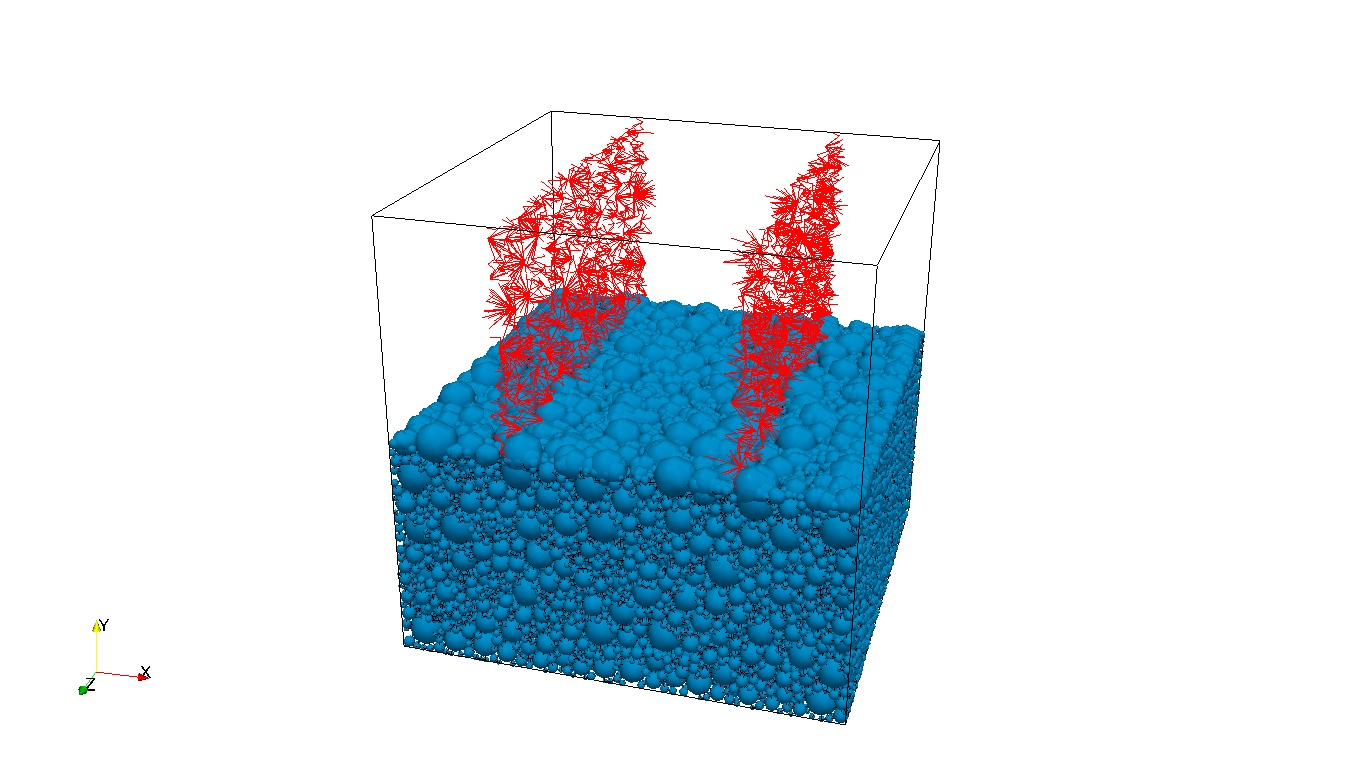
\includegraphics[scale=0.12]{./figures/frac2.jpg}}
\subfigure[4 fractures]{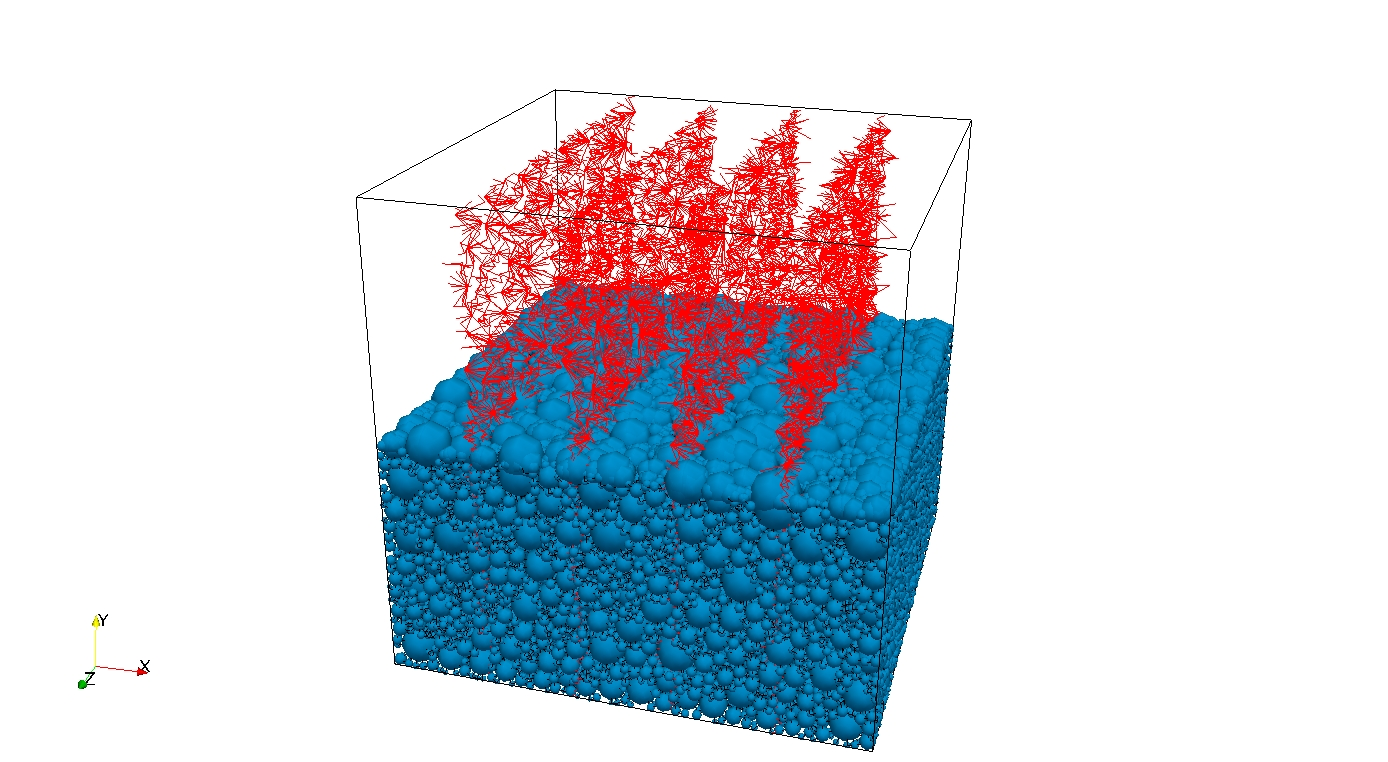
\includegraphics[scale=0.115]{./figures/frac4.jpg}}
\centering
\caption{Fractures (represented by the red colour) inside the medium}\label{FIG:GEOMETRY}
\end{figure}


\subsection{Porosity and Elastic Tensor}\label{SEC:PORO}
Among a few factors that affect the elastic tensor of the coal matrix, the coal porosity plays an important role. In this section, we first study the porosity effect on the evalution of elastic tensor. In DEM modelling, the matrix porosity is largely determined by the particle sizes. Table~ \ref{TABLE:POROSITY} compares the weakness of coal matrix regarding different porosity settings.

Moreover, Figure~\ref{FIG:POROSITY} desplays the distribution of stress-strain under different porosities.

NOTE: here illustrates the figure.

\begin{table}
\centering
\caption{Model calibration results. $E_{mac}$ and $\nu_{mac}$ are referring to macroscopic Young's modulus and Poisson's ratio, respectively. }
\begin{threeparttable}[b]
\begin{tabular} {lrrrrrrrr}
%\begin{tabular}{p{2cm}p{4cm}p{4cm}}
\hline\hline 
 \multicolumn{9}{c}{Isotropic sample} \\
 \hline
Value\tnote{1} & $C_{11}$ & $C_{12}$ &  $C_{23}$ & $C_{33}$ & $C_{44}$ & $C_{66}$ & $E_{mac}$ & $\nu_{mac}$\\
\hline
$\phi=$ 		& 1.309 & 0.613 \\
$\phi=$  		& 0.587 & 0.269 \\
$\phi=$  		& 0.587 & 0.269 \\
$\phi=$ 		& 1.309 & 0.613 \\
$\phi=$ 		& 0.361 & 0.172 \\
$\phi=$ 		& 0.361 & 0.172 \\
$\phi=$   	    & 0.946 & 0.449 \\
$\phi=$ 	  	& 0.310 & 0.305 \\
$\phi=$ 		& 1.309 & 0.613 \\
$\phi=$  		& 0.587 & 0.269 \\
$\phi=$  		& 0.587 & 0.269 \\
$\phi=$ 		& 1.309 & 0.613 \\
$\phi=$ 		& 0.361 & 0.172 \\
\hline    
\bottomrule
\end{tabular}\label{TABLE:POROSITY}
\begin{tablenotes}
      \small
      \item [1] The unit for $C_{ij}$ and $E_{mac}$ is $MPa$.
	\end{tablenotes}
\end{threeparttable}
\end{table}


\begin{figure}
\includegraphics[scale=0.8]{./figures/porosity.jpg}
\centering
\caption{Stress-strain of isotropic sample under different matrix porosities}\label{FIG:POROSITY}
\end{figure}

\subsection{Fractured Media}\label{SEC:FRAC}

In Equation~(\ref{EQ:DELTAN}) and~(\ref{EQ:DELTAT}), macroscopic parameters $M'$, $\mu'$, and fracture properties (e.g., $a/c$ and $e$) all affect the normal and tangential weakness $\Delta_N$ and $\Delta_T$. In this section, we compare the impact of fracture density and fractured-filled materials on the elasticity tensor.
In accordance with Linear-slip models it is assumed that 
fractures are independent, oriented parallel to the $x_{2}x_{3}$ plane, see Figure~\ref{FIG:FRACS}. 
In this initial test we consider the three cases of 8 fractures (Figure~\ref{FIG:FRACSa}), 
64 fractures (Figure~\ref{FIG:FRACSb}) and 4 fractures, see Figure~\ref{FIG:FRACSc}.

For 8 fractures, the semi-major and semi-minor axes of each fracture are set to $a=4mm$ and $c=2mm$, respectively. 
The distance ($\Delta D$) between two adjacent parallel fractures is $25mm$. For 64 fractures, $a=2 mm$, $c=1 mm$ and $\Delta D = 1.25cm$. 
For both cases the fracture density is calculated as $e = 6.43{\times}10^{-3}$. For four fractures, we choose $a=20mm$, $c=2mm$ and $\Delta D =12.5mm$. In this case the fracture density $e=8.04{\times}10^{-2}$ that is over one order of magnitude higher than the fracture densities for the two other cases. 

\begin{figure}
\subfigure[Uni-axial, $8$ fractures]{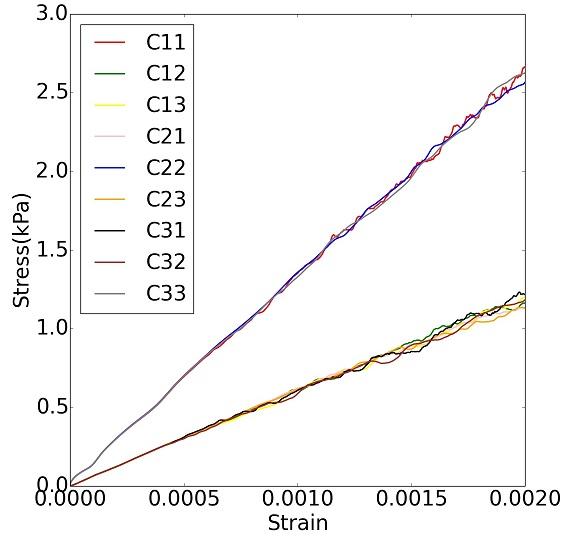
\includegraphics[scale=0.35]{./figures/frac8-some-low.jpg}\label{FIG:FRACS-Fluida}}
\subfigure[Shear, $8$ fractures ]{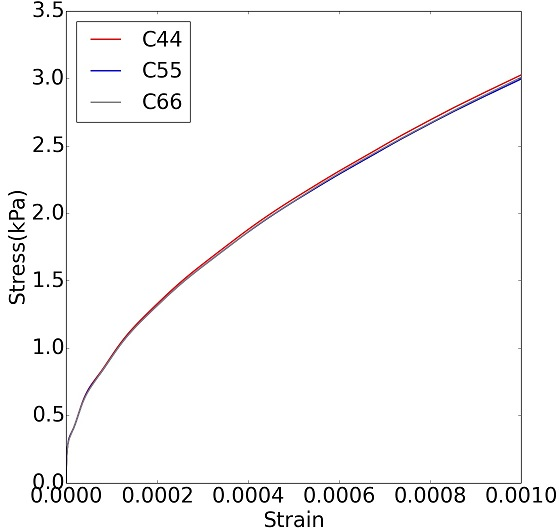
\includegraphics[scale=0.35]{./figures/frac8-some-low-shear.jpg}\label{FIG:FRACS-Fluidb}}
\subfigure[Uni-axial, $64$ fractures ]{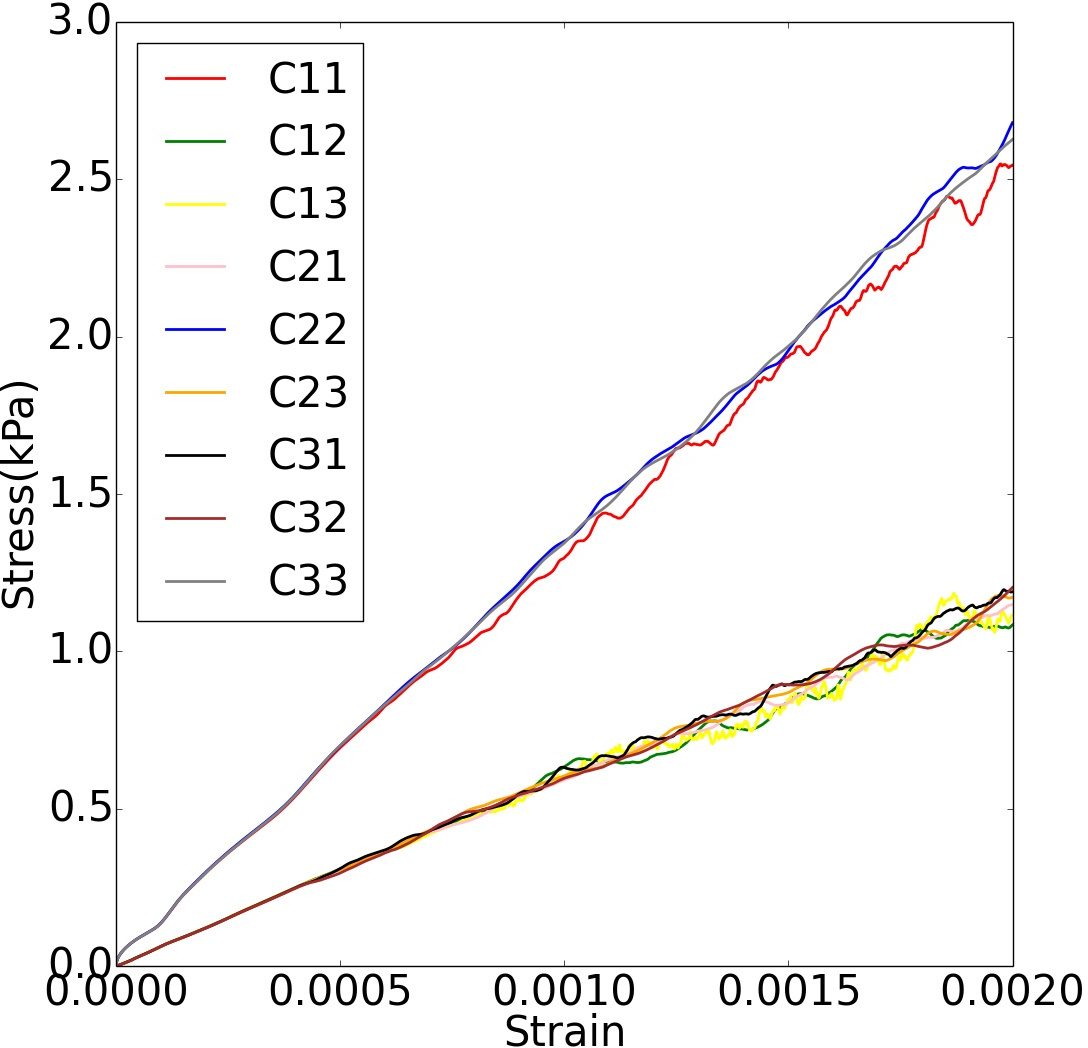
\includegraphics[scale=0.133]{./figures/frac64-some-low.jpg}\label{FIG:FRACS-Fluidc}}
\subfigure[Shear, $64$ fractures ]{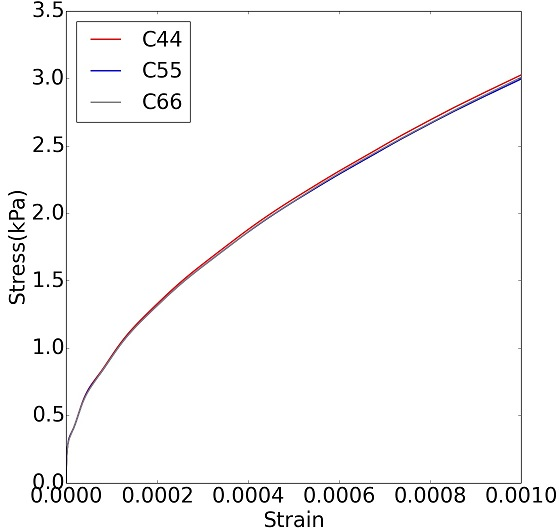
\includegraphics[scale=0.35]{./figures/frac64-some-low-shear.jpg}\label{FIG:FRACS-Fluidd}}
\subfigure[Uni-axial, $4$ fractures ]{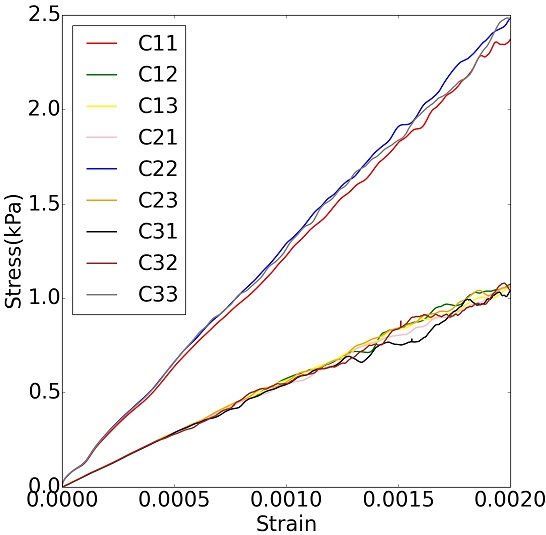
\includegraphics[scale=0.35]{./figures/frac4-some-low.jpg}\label{FIG:FRACS-Fluide}}
\subfigure[Shear, $4$ fractures ]{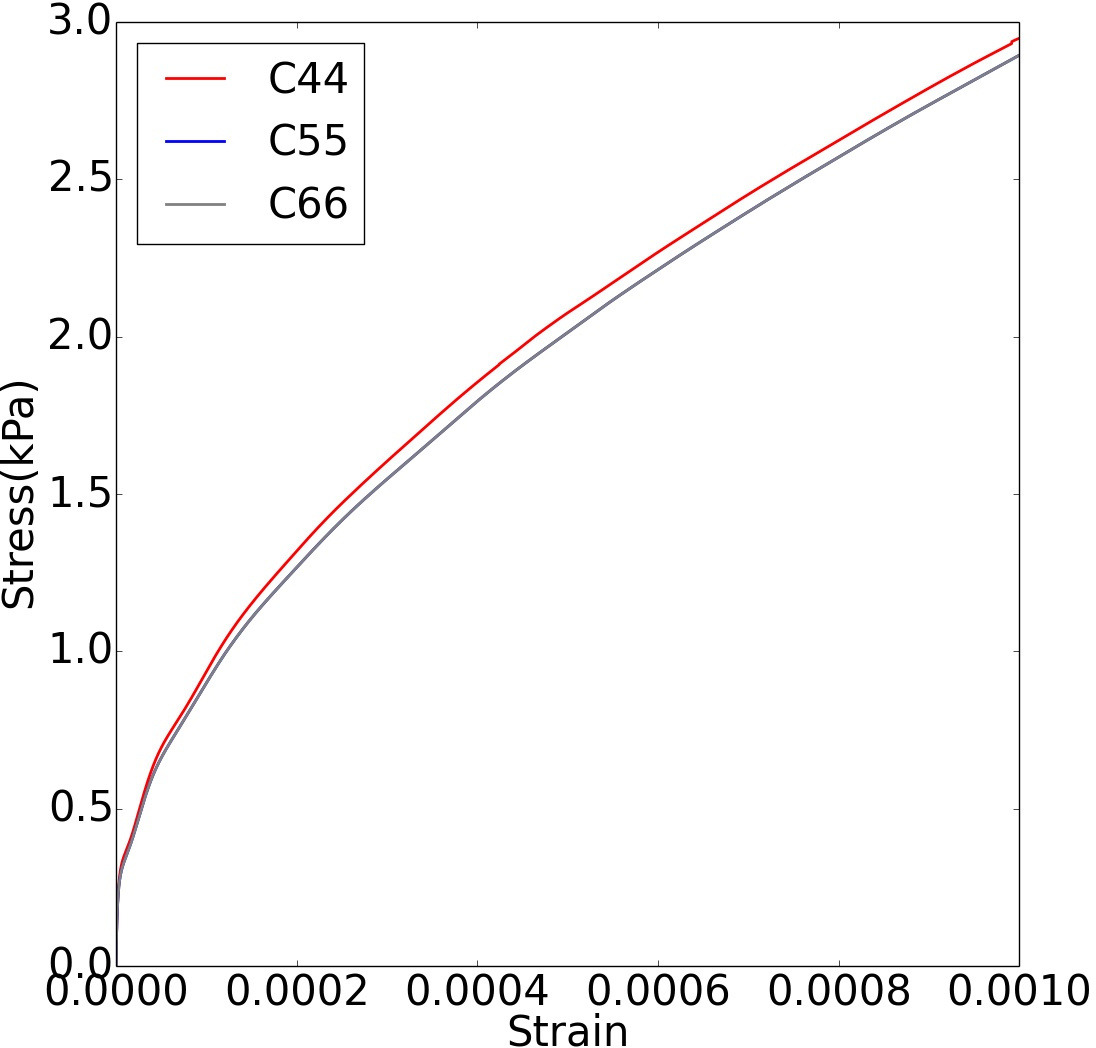
\includegraphics[scale=0.133]{./figures/frac4-some-low-shear.jpg}\label{FIG:FRACS-Fluidf}}
\centering
\caption{Stress-strain of fractured sample with filling material $E'_{dem} = 1.5 MPa$ and $\nu'_{dem} = 0.25$ }\label{FIG:FRACS-Fluid}
\end{figure}

\begin{sidewaystable}
\centering
\begin{threeparttable}
\caption{Elastic tensor entries and Thomsen-style parameters with filling material $E'_{dem} = 1.5 MPa$ and $\nu'_{dem} = 0.25$.}
\begin{tabular}{lrr|rr|rr}
%{p{1cm}p{1.7cm}p{1.5cm}|p{1.7cm}p{1.5cm}|p{1.7cm}p{1.5cm}}
\hline\hline
& \multicolumn{2}{c|}{$8$ fractures}& \multicolumn{2}{c|}{$64$ fractures } & \multicolumn{2}{c}{$4$ fractures}\\
\hline
Value\tnote{1} & Linear-slip & DEM & Linear-slip & DEM & Linear-slip & DEM\\
\hline
$C_{11}$ 		& 1.305 & 1.305 & 1.305 & 1.305 & 1.260 & 1.200 \\
$C_{12}$ 		& 0.585 & 0.585 & 0.585 & 0.585 & 0.565 & 0.543 \\
$C_{23}$ 		& 0.586 & 0.586 & 0.586 & 0.586 & 0.577 & 0.551 \\
$C_{33}$ 		& 1.308 & 1.308 & 1.308 & 1.308 & 1.300 & 1.243 \\
$C_{44}$ 		& 0.361 & 0.361 & 0.361 & 0.361 & 0.361 & 0.361 \\
$C_{66}$ 		& 0.356 & 0.356 & 0.356 & 0.356 & 0.298 & 0.263 \\
$\Delta_N$  	& $3.02{\times}10^{-3}$ & $3.05{\times}10^{-3}$ & $3.02{\times}10^{-3}$ & $3.05{\times}10^{-3}$ & $3.77{\times}10^{-2}$ & $8.33{\times}10^{-2}$ \\
$\Delta_T$	    & $1.40{\times}10^{-2}$ & $1.39{\times}10^{-2}$ & $1.40{\times}10^{-2}$ & $1.41{\times}10^{-2}$ & $0.175$ & $0.271$ \\
$\varepsilon^{(2)}$ & $-1.21{\times}10^{-3}$ & $-1.15{\times}10^{-3}$ & $-1.21{\times}10^{-3}$ & $-1.15{\times}10^{-3}$ & $-1.52{\times}10^{-2}$ & $-0.173$  \\
$\gamma^{(2)}$  & $-7.01{\times}10^{-3}$ & $-6.92{\times}10^{-3}$ & $-7.01{\times}10^{-3}$ &  $-7.07{\times}10^{-3}$ & $-8.76{\times}10^{-2}$ & $-0.136$ \\
$\delta^{(2)}$ & $-7.46{\times}10^{-4}$ & $-7.64{\times}10^{-4}$ & $-7.46{\times}10^{-4}$ & $-7.64{\times}10^{-4}$ & $-9.33{\times}10^{-3}$ & $-1.79{\times}10^{-2}$ \\
\hline    
\bottomrule
\end{tabular}\label{TABLE:DENSITY}
\begin{tablenotes}
  \item [1] The unit for $C_{ij}$ is $MPa$.
\end{tablenotes}
\end{threeparttable}
\end{sidewaystable}

%In all three cases, fractures are filled with a material with local %elasticity parameters as $E'_{dem}= 1.5 MPa$ and $\nu'_{dem} = 0.25$. 
%Porosity is chosen to the same value as the background media ($\phi=0.23$), %so local elastic parameters can be used in 
%equations~(\ref{EQ:DELTAN}) and~(\ref{EQ:DELTAT}). Elastic parameters are %calculated with the unconfined, uni-axial compression 
%and shear tests in Figure~\ref{FIG:FRACS-Fluid}.  For details, values for %elasticity parameters, weakening factors and Thomsen-style parameters
%are shown in Table~\ref{TABLE:DENSITY}. For the cases of $8$ and $64$ %fractures, the Linear-slip models and the DEM model are in good 
%agreement even for the weakening factors that are small perturbations to the %isotropic elasticity parameters only. It is pointed 
%out in this case the fracture density and the ratios of semimajor and %semiminor axes are identical. Hence, the Linear-slip models predicts %identical anisotropy properties for these two cases. 
%For the four fractures case the Hudson's model and the DEM model predict the %same order of magnitude for the tangential and normal weaknesses
%but the actually values diverge where the DEM predict a much higher weakness. %We attribute this to fact that the fundamental assumption of non-interacting %fractures for the Hudon's model is not applicable for this case. 
%The significant difference on the Thomson-style parameters is highlighted. In %particular, the DEM predicts a much higher values for $\varepsilon^{(2)}$ %that is relevant for non-hyperbolic NMO analysis.
%It is certainly arguable if the four fracture case represents a realistic %fracture configuration but the test gives an indication that for interacting %fractures scenarios fracturing leads to much higher Thomson-style parameters %than predicted Hudson's model.


\begin{figure}
\subfigure[Uni-axial, $8$ fractures]{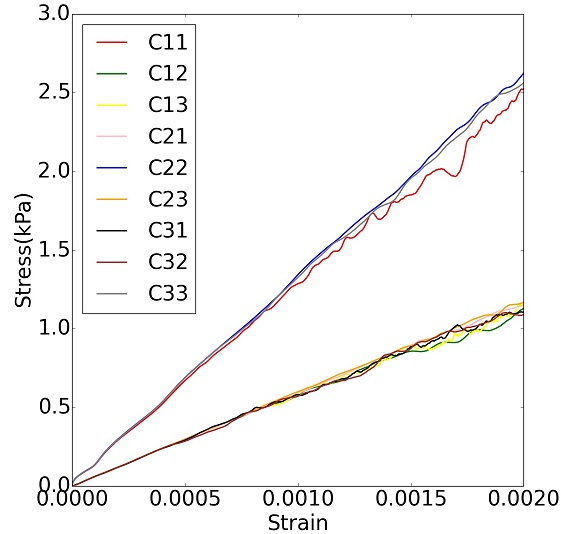
\includegraphics[scale=0.35]{./figures/frac8-0-low.jpg}}
\subfigure[Shear, $8$ fractures]{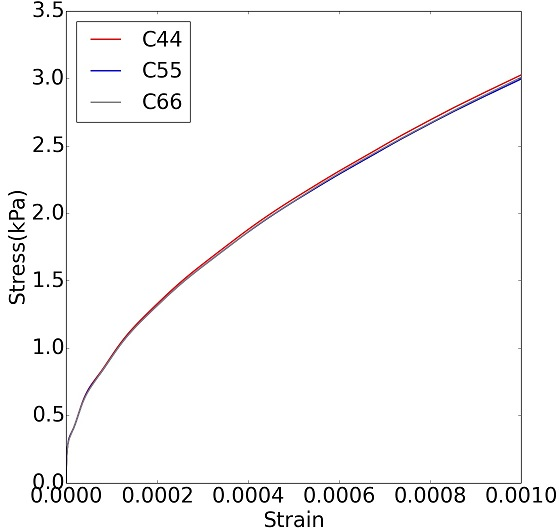
\includegraphics[scale=0.35]{./figures/frac8-0-low-shear.jpg}}
\subfigure[Uni-axial, $64$ fractures]{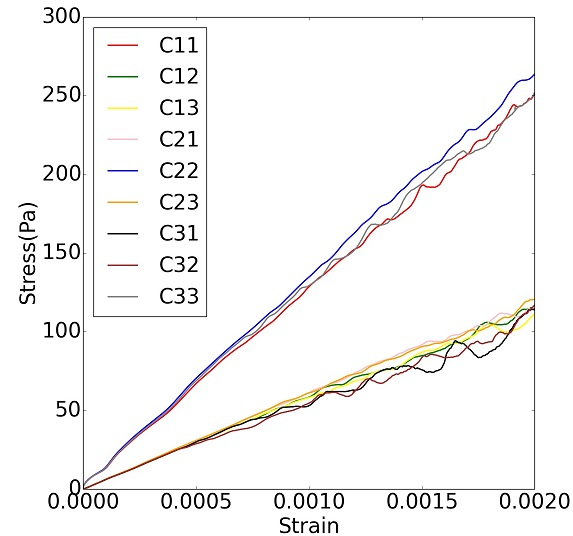
\includegraphics[scale=0.35]{./figures/frac64-0-low.jpg}}
\subfigure[Shear, $64$ fractures]{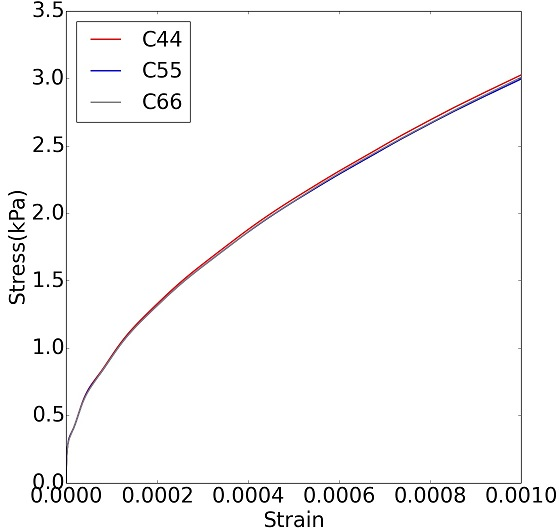
\includegraphics[scale=0.35]{./figures/frac64-0-low-shear.jpg}}
\subfigure[Uni-axial, $4$ fractures]{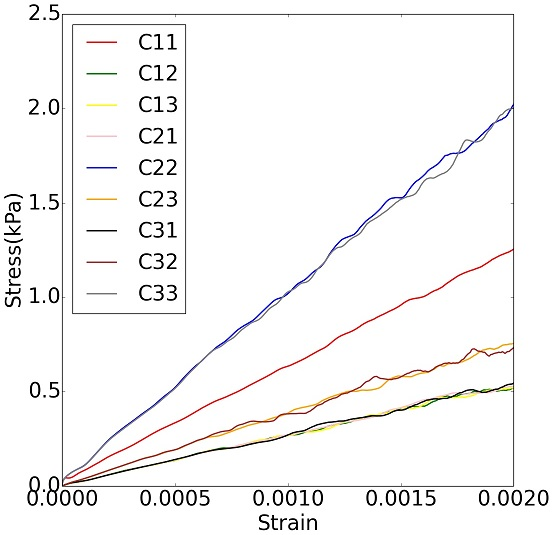
\includegraphics[scale=0.35]{./figures/frac4-0-low.jpg}}
\subfigure[Shear, $4$ fractures]{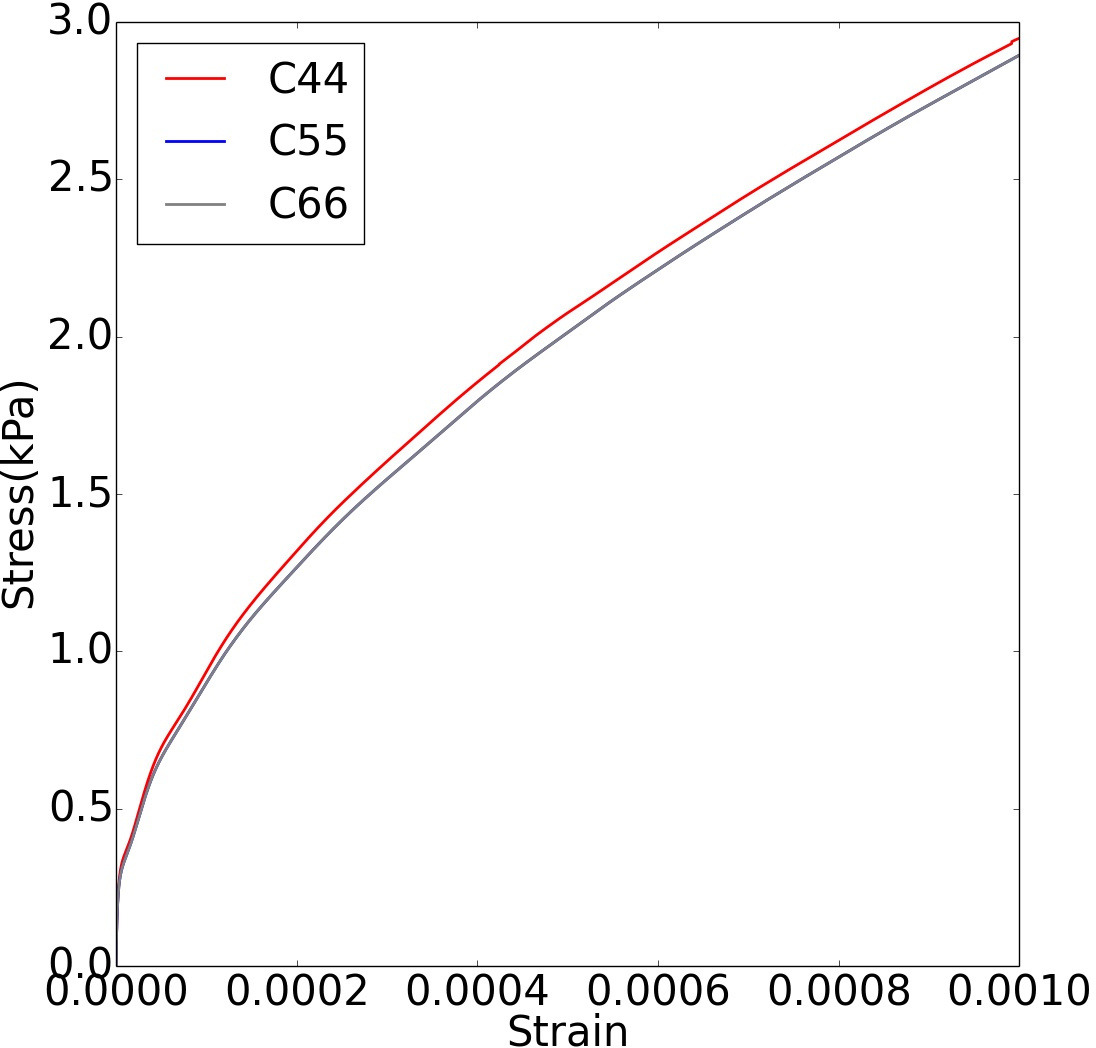
\includegraphics[scale=0.133]{./figures/frac4-0-low-shear.jpg}}
\centering
\caption{Stress-strain of fractured sample with filling material $E'_{dem} = 0 MPa$.}\label{FIG:FRACS-DRY}
\end{figure}

\begin{sidewaystable}
\centering
\begin{threeparttable}
\caption{Elastic tensor entries and Thomsen-style parameters with filling material $E'_{dem} = 0 MPa$.}
\begin{tabular}{lrr|rr|rr}
 \hline
& \multicolumn{2}{c|}{8 fractures}& \multicolumn{2}{c|}{64 fractures} & \multicolumn{2}{c}{4 fractures}\\
\hline
Value\tnote{1} & Linear-slip & DEM & Linear-slip & DEM & Linear-slip & DEM\\
\hline
$C_{11}$ 		& 1.253 & 1.253 & 1.253 & 1.253 & 0.606 & 0.618 \\
$C_{12}$ 		& 0.562 & 0.563 & 0.562 & 0.563 & 0.272 & 0.277 \\
$C_{23}$ 		& 0.576 & 0.577 & 0.576 & 0.577 & 0.446 & 0.383 \\
$C_{33}$ 		& 1.298 & 1.298 & 1.298 & 1.298 & 1.168 & 1.001 \\
$C_{44}$ 		& 0.361 & 0.361 & 0.361 & 0.361 & 0.361 & 0.361 \\
$C_{66}$ 		& 0.356 & 0.356 & 0.356 & 0.356 & 0.298 & 0.263 \\
$\Delta_N$  	& $4.30{\times}10^{-2}$ & $4.28{\times}10^{-2}$ & $4.30{\times}10^{-2}$ & $4.31{\times}10^{-2}$ & 0.537 & 0.528 \\
$\Delta_T$	& $1.40{\times}10^{-2}$ & $1.40{\times}10^{-2}$ & $ 1.40{\times}10^{-2}$ & $1.43{\times}10^{-2}$ & 0.175 & 0.271 \\
$\varepsilon^{(2)}$ & $-1.73{\times}10^{-2}$ & $-1.73{\times}10^{-2}$ & $-1.73{\times}10^{-2}$ & $-1.73{\times}10^{-2}$ & $-0.240$ & $-0.191$ \\
$\gamma^{(2)}$ 	  & $-7.01{\times}10^{-3}$ & $-6.93{\times}10^{-3}$ & $-7.01{\times}10^{-3}$ & $-6.93{\times}10^{-3}$ & $-8.76{\times}10^{-2}$ & $-0.136$ \\
$\delta^{(2)}$      & $-1.06{\times}10^{-2}$ & $-9.95{\times}10^{-3}$ & $-1.06{\times}10^{-2}$ & $-9.99{\times}10^{-3}$ & $-0.133$ & $-2.01{\times}10^{-3}$ \\
\hline    
\bottomrule
\end{tabular}\label{TABLE:DRY}
\begin{tablenotes}
      \item [1]  The unit for $C_{ij}$ is MPa.
\end{tablenotes}
\end{threeparttable}
\end{sidewaystable}

\begin{sidewaystable}
\centering
\begin{threeparttable}
\caption{Elastic tensor entries and Thomsen-style parameters with filling material $E'_{dem} = 0 MPa$.}
\begin{tabular}{lrr|rr|rr}
 \hline
& \multicolumn{2}{c|}{8 fractures}& \multicolumn{2}{c|}{64 fractures} & \multicolumn{2}{c}{4 fractures}\\
\hline
Value\tnote{1} & Linear-slip & DEM & Linear-slip & DEM & Linear-slip & DEM\\
\hline
$C_{11}$ 		& 1.253 & 1.253 & 1.253 & 1.253 & 0.606 & 0.618 \\
$C_{12}$ 		& 0.562 & 0.563 & 0.562 & 0.563 & 0.272 & 0.277 \\
$C_{23}$ 		& 0.576 & 0.577 & 0.576 & 0.577 & 0.446 & 0.383 \\
$C_{33}$ 		& 1.298 & 1.298 & 1.298 & 1.298 & 1.168 & 1.001 \\
$C_{44}$ 		& 0.361 & 0.361 & 0.361 & 0.361 & 0.361 & 0.361 \\
$C_{66}$ 		& 0.356 & 0.356 & 0.356 & 0.356 & 0.298 & 0.263 \\
$\Delta_N$  	& $4.30{\times}10^{-2}$ & $4.28{\times}10^{-2}$ & $4.30{\times}10^{-2}$ & $4.31{\times}10^{-2}$ & 0.537 & 0.528 \\
$\Delta_T$	& $1.40{\times}10^{-2}$ & $1.40{\times}10^{-2}$ & $ 1.40{\times}10^{-2}$ & $1.43{\times}10^{-2}$ & 0.175 & 0.271 \\
$\varepsilon^{(2)}$ & $-1.73{\times}10^{-2}$ & $-1.73{\times}10^{-2}$ & $-1.73{\times}10^{-2}$ & $-1.73{\times}10^{-2}$ & $-0.240$ & $-0.191$ \\
$\gamma^{(2)}$ 	  & $-7.01{\times}10^{-3}$ & $-6.93{\times}10^{-3}$ & $-7.01{\times}10^{-3}$ & $-6.93{\times}10^{-3}$ & $-8.76{\times}10^{-2}$ & $-0.136$ \\
$\delta^{(2)}$      & $-1.06{\times}10^{-2}$ & $-9.95{\times}10^{-3}$ & $-1.06{\times}10^{-2}$ & $-9.99{\times}10^{-3}$ & $-0.133$ & $-2.01{\times}10^{-3}$ \\
\hline    
\bottomrule
\end{tabular}\label{TABLE:DRY}
\begin{tablenotes}
      \item [1]  The unit for $C_{ij}$ is MPa.
\end{tablenotes}
\end{threeparttable}
\end{sidewaystable}

In a second series of tests we investigate the impact of the filling material. To simulate a gas filling of the fracture we set $E'_{dem} = 0 MPa$ and $\nu'_{dem} = 0$ 
(the value of the latter is in fact irrelevant). The strain-stress response curves for the three fracture configurations as discussed before 
are shown in Figure~\ref{FIG:FRACS-DRY}. Table~\ref{TABLE:DRY} compares the results of the Linear-slip models and DEM simulation. 
Again we see a very good agreement for the sparse fracture distribution ($8$ and $64$ fractures). 
For the high density case of $4$ fractures both models show strong weaknesses normal to the fault where values are in good agreement. 
Again values for the normal weakness diverge but - as predicted by the Linear-slip models - are not influenced by the fracture filling under the 
investigated configuration. Values for $\varepsilon^{(2)}$ are in better agreement now. We point out the disagreement in $\delta^{(2)}$  which
is relevant for azimuthal hyperbolic NMO analysis. While the Linear-slip models predict significant flatness in the NMO velocity ellipse, the DEM predicts a signficant less eccentric ellipse for this case of interacting fractures. 

\subsection{Fractured Media from micro-CT Scans}\label{SEC:FRAC}

\section{Conclusions}\label{SEC:CONCL}
%In the paper, we tested the DEM model for the elastic properties of a %fractured medium against the well-established Hudson's model. 
%For sparse, non-interacting fractures tangential and normal weaknesses of the %DEM model and Hudson's model are in good agreement. This is despite the fact %that in the scenarios tested weaknesses due to fracturing were well below $1 %\%$ of the  fractured background media and hence difficult to be separated %form the background elastic properties. The test shown also indicate that %this result is robust with the fracture filling.

%We also showed results for a case of high fracture density violating the %assumption of non-interacting fractures used in the Hudson's model. The
%setup investigation does not necessarily represent a realistic scenario. %However, the tests show that the assumption of non-interacting fractures is %vital to bring the DEM and the Hudson's model to agreement. 
%The tests also indicate that for dense, interacting fractures, the Hudson and %DEM model show significant different values for the Thomsen-style parameters %for azimuthal hyperbolic as well as non-hyperbolic NMO analysis. This %requires different interpretation of anisotropy parameters in highly %fractured systems such as coal. To what extend this result applies to more %realistic fracture set-ups is currently under investigations using DEM %simulation.

\section{Acknowledgements}
This research was financially supported by industry funding provided via The University of Queensland Centre for Coal Seam Gas (\url{www.ccsg.uq.edu.au}) and the AuScope National Collaborative Research Infrastructure Strategy (NCRIS).

\section*{References}
\bibliographystyle{elsarticle-num-names} 
\bibliography{./mybibfile}

\end{document}
\endinput
%%
%% End of file `elsarticle-template-num.tex'.
